\documentclass{beamer}
\usetheme{Madrid}

\usepackage{amsmath}
\usepackage{graphicx}

\usepackage{tikz}

\usepackage[justification=centering]{caption}
\usepackage{subcaption}

\usepackage{xurl}

% default path to images and other assets
\graphicspath{{assets/}}

% disable wrapping
\tolerance=1
\emergencystretch=\maxdimen
\hyphenpenalty=10000
\hbadness=10000

% number figure caption
\setbeamertemplate{caption}[numbered]

% display bib label in references
\setbeamertemplate{bibliography item}{\insertbiblabel}
\setbeamertemplate{bibliography entry title}{}
\setbeamertemplate{bibliography entry location}{}
\setbeamertemplate{bibliography entry note}{}

% Metadata
% ------------------------
\title[Instance segmentation]{Instance segmentation of biomedical images with an object-aware
embedding learned with local constraints}
\subtitle{Seminar Computational Life Science}

\author[Oleh Shkalikov]{Oleh Shkalikov \texorpdfstring{\\ 5102818}{}}

\institute[TU Dresden]{TU Dresden, Computer Science Faculty}

\date{9 May, 2023}

% ------------------------

\begin{document}

\frame{\titlepage}

\begin{frame}
    \frametitle{Agenda}
    \tableofcontents
\end{frame}

\section{Problem formulation}

\begin{frame}
    \frametitle{Instance Segmentation}

\end{frame}

\begin{frame}
    \frametitle{Semantic VS Instance Segmentation}

    \begin{figure}[h]
        \begin{subfigure}{0.5\textwidth}
            \centering
            \includegraphics[width=0.95\textwidth]{semantic_segm_example.png}
            \caption{Semantic segmentation}
        \end{subfigure}
        \begin{subfigure}{0.49\textwidth}
            \centering
            \includegraphics[width=0.95\textwidth]{instance_segm_example.png}
            \caption{Instance segmentation}
        \end{subfigure}
        \caption{Comparison of the different segmentation types. Source publication is \cite{segm_type_comp}}.
    \end{figure}

\end{frame}

\begin{frame}
    \frametitle{Metric}

\end{frame}

\section{Previous approaches}

\begin{frame}
    \frametitle{Approaches to Solve the Problem}

    \centering
    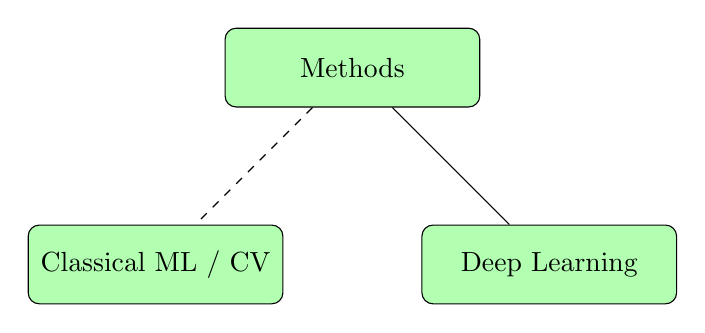
\begin{tikzpicture}[nodes={rectangle, rounded corners, minimum width=3cm, text width=3cm, minimum height=1cm,text centered, draw=black, fill=green!30},
            sibling distance=5cm, level distance=2.5cm]
        \node {Methods}
        child {node(a){Classical ML / CV} edge from parent [dashed]}
        child {node(b){Deep Learning}};
    \end{tikzpicture}

    \vspace*{0.5cm}
    \begin{block}{Why Deep Learning?}
        Neural networks significantly outperforms all classical
        methods because they can be represented as a learnable feature
        extractor and regressor or classification head. Whereas classical approaches are
        based on hand-made or fixed features which are hard to derive and not flexible.
    \end{block}

\end{frame}

\begin{frame}
    \frametitle{Neural Network Building Blocks}

    \begin{figure}[h]
        \begin{subfigure}[t]{0.5\textwidth}
            \centering
            \includegraphics[width=0.85\textwidth]{conv2d.pdf}
            \caption{Padded 2D Convolution. Source: \cite{zhang2021dive}}
        \end{subfigure}
        \begin{subfigure}[t]{0.49\textwidth}
            \centering
            \includegraphics[width=0.8\textwidth]{pooling.pdf}
            \caption{Max Pooling. Source: \cite{zhang2021dive}}
        \end{subfigure}
        \begin{subfigure}{0.5\textwidth}
            \centering
            \includegraphics[width=0.8\textwidth]{upsampling.png}
            \caption{Nearest Neighbour Upsampling. Source: \cite{phdthesis}}
        \end{subfigure}
        \begin{subfigure}{0.49\textwidth}
            \centering
            \includegraphics[width=0.9\textwidth]{dropout.pdf}
            \caption{Dropout (1 dim case). Source: \cite{zhang2021dive}}
        \end{subfigure}
        \caption{Basic building blocks of CNNs}.
    \end{figure}

\end{frame}

\begin{frame}
    \frametitle{UNet}

    \begin{figure}[h]
        \includegraphics[width=0.8\textwidth]{unet.png}
        \caption{Original UNet architecture from \cite{ronneberger2015u}}
    \end{figure}

\end{frame}

\begin{frame}
    \frametitle{Mask R-CNN}

    \begin{block}{Two stage}
        Mask R-CNN is a two stage architecture: region proposal
        and classification with segmentation / bounding box refinement.
    \end{block}

    \begin{figure}[h]
        \begin{subfigure}{0.65\textwidth}
            \includegraphics[width=\textwidth]{mask_rcnn.png}
            \caption{Mask R-CNN pipeline}
        \end{subfigure}
        \begin{subfigure}{0.34\textwidth}
            \includegraphics[width=\textwidth]{roi_align.png}
            \caption{ROI align}
        \end{subfigure}
        \caption{Mask R-CNN architecture \cite{he2017mask}}
    \end{figure}

\end{frame}

\begin{frame}
    \frametitle{Stardist}

    \begin{block}{Idea of Stardist}
        A model is trained to densely predict the distances ($r$)
        to the object boundary \textbf{along a fixed set of rays} and object
        probabilities ($d$), which together produce an
        overcomplete set of candidate polygons for a given
        input image. The final result is obtained via
        non-maximum suppression of these candidates.
    \end{block}

    \begin{figure}[h]
        \includegraphics[width=\textwidth]{stardist.png}
        \caption{Stardist explanation. Source: \cite{schmidt2018}}
    \end{figure}

\end{frame}

\begin{frame}
    \frametitle{Previous Works Summary}

    \begin{itemize}[<+->]
        \item Sematic segmentation based method predicts contours $\implies$
              few misclassified pixel ends up with one big connected region crowded objects
        \item Approaches which are using NMS, like Mask R-CNN, suppress objects when their bounding boxes
              overlap with a large ratio
        \item Stardist is suitable only for fixed shape objects
    \end{itemize}

\end{frame}

\section{Proposed method}

\begin{frame}
    \frametitle{Network architecture}

    \begin{block}{Idea}
        Compute pixel-wise embeddings which will be similar within the
        object but orthogonal for every two \textbf{neighboring} objects.
    \end{block}

    \begin{figure}[h]
        \includegraphics[height=0.49\textheight]{obj_aware_arch.png}
        \caption{Proposed architecture with 2 heads: for distance to boundary
            regression and embeddings. Source: \cite{chen2019instance}}
    \end{figure}

\end{frame}

\begin{frame}
    \frametitle{Actual Implementation}

    \begin{alertblock}{Difference in paper and official implementation}
        In official implementation authors use UNet like architecture, but starting with
        the first upsampling block they use different layers for distance regressor and
        embeddings.
    \end{alertblock}

    \begin{figure}[h]
        \includegraphics[height=0.43\textheight]{net_impl.png}
        \caption{Actual network implementation. Source: \url{https://github.com/looooongChen/instance_segmentation_with_pixel_embeddings}}
    \end{figure}

\end{frame}

\begin{frame}
    \frametitle{Loss function}

    Total loss is a sum of 2 losses (here $\lambda = 5$)
    \[
        L = L_{reg} + \lambda L_{emb}
    \]

    Suppose there are $K$ objects within an image with ($M_1$, $M_2$, $\dots$ , $M_K$ )
    pixels respectively and the cosine distance denoted as $D$, then
    \[
        L_{reg} = \frac{1}{\sum\limits_{k=1}^K M_k} \sum\limits_{k=1}^K \sum\limits_{p=1}^{M_k} w_p (d_p - \hat{d_p})^2
    \]
    \[
        L_{emb} = \frac{1}{\sum\limits_{k=1}^K M_k} \sum\limits_{k=1}^K \sum\limits_{p=1}^{M_k} w_p D(e_p, u_k) +
        \frac{1}{K} \sum\limits_{k=1}^K \frac{1}{|N_d(k)|} \sum\limits_{n \in N_d(k)} |1 - D(e_p, u_k)|
    \]
    where $d_p$ and $\hat{d_p}$ -- reg. output and ground truth of $p$, $e_p$ --
    embedding of $p$, $u_k$ -- mean embedding of object $k$,
    $w_p$ -- foreground / background weight. $N_d(k)$ -- $d$-neighborhood of object $k$.

\end{frame}

\begin{frame}
    \frametitle{Postprocessing}

    \begin{enumerate}
        \item Threshold the distance map to get the central region of an object. Authors use $T_c = 0.7$ in their experiment.
        \item Compute the mean embedding $u_k$ of each seed region.
        \item Iteratively perform morphological dilation with a $3 \times 3$ kernel.
              Frontier pixels $e_i$ are included into the object, if it is not assigned to other objects and
              $D(e_i, u_k)$ is smaller than $T_e = 0.3$.
        \item Stop when no new pixels are included.
    \end{enumerate}

    \begin{exampleblock}{Alternative}
        Mean-shift, graph watershed, other clustering methods that
        does not require to specify the number of clusters
    \end{exampleblock}

\end{frame}

\section{Analysis of the performance}

\begin{frame}
    \frametitle{Qualitative results }

    Datasets which have been used for evaluation:
    \begin{itemize}
        \item Cells: sampled 1233 images from BBBC006+partDSB2018
        \item Leaves: sampled 810 images from CVPPP2017
    \end{itemize}

    \begin{figure}[h]
        \includegraphics[height=0.5\textheight]{results_pict_comp.png}
        \caption{Comparison of different method on datasets.
            In the first row, correct matches (IoU = 0.6) are highlighted in
            blue, while false positives are marked in red. The second row shows the leaf
            segmentation results with color-coded instances}
    \end{figure}

\end{frame}

\begin{frame}
    \frametitle{Leaf Dataset Metrics}

    \begin{table}
        \small
        \begin{tabular}[pos]{*{5}{c}}
            \hline
            Metric                                                                     & SBD             & FBD             & DiC              & $|$DiC$|$       \\
            \hline
            Unet9\footnote{simplified: 3 down and 3 up}                                & 0.5456          & 0.9045          & -3.9259          & 5.0370          \\
            Stardist                                                                   & 0.8019          & 0.9327          & 1.9506           & 2.6543          \\
            Mask-RCNN\footnote{fine-tuned, pretrained on MS COCO}                      & 0.7972          & 0.9060          & -0.1543          & 1.080           \\
            \hline
            d10-dim16\footnote{$d$ -- neighborhood size, $dim$ -- embedding dimension} & \textbf{0.8307} & \textbf{0.9417} & \textbf{-0.1790} & \textbf{0.7346} \\
            d30-dim16                                                                  & 0.8159          & 0.9303          & -0.2160          & 0.7593          \\
            d100-dim16                                                                 & 0.8101          & 0.9312          & -0.2593          & 0.9259          \\
            \hline
            d10-dim4                                                                   & 0.8005          & 0.9377          & -0.6605          & 1.0185          \\
            d30-dim4                                                                   & 0.7163          & 0.3338          & -0.6358          & 0.9444          \\
            d100-dim4                                                                  & 0.7095          & 0.3495          & -0.5432          & 1.0741          \\
            \hline
        \end{tabular}
        \caption{Value of metrics on the leaves dataset}
    \end{table}

    \vspace*{-0.5cm}
    \begin{itemize}
        \item Embeddings matter: low embedding dimension
              - bad metric's value
        \item Local better than global, because using embedding space
              efficiently
    \end{itemize}

\end{frame}

\begin{frame}
    \frametitle{Cell Dataset Metrics}

    \begin{table}
        \scalebox{0.7}
        {
            \begin{tabular}[pos]{*{11}{c}}
                \hline
                \textit{IoU} & 0.5            & 0.55           & 0.6            & 0.65           & 0.7            & 0.75           & 0.8            & 0.85           & 0.9            & mean AP        \\
                \hline
                UNet         & .8302          & .8152          & .7994          & .7816          & .7609          & .7206          & .6216          & .4478          & .2332          & .6678          \\
                Stardist     & .8178          & .8015          & .7880          & .7733          & .7552          & .7304          & .6910          & .6225          & .4749          & .7172          \\
                Mask-RCNN    & .8820          & .8636          & .8492          & .8354          & \textbf{.8231} & \textbf{.8030} & \textbf{.7728} & \textbf{.7095} & .5483          & \textbf{.7874} \\
                \hline
                d10-dim16    & \textbf{.9108} & \textbf{.8858} & \textbf{.8611} & \textbf{.8428} & .7936          & .7518          & .7031          & .6466          & \textbf{.5528} & .7720          \\
                d30-dim16    & .9039          & .8727          & .8480          & .8169          & .7776          & .7305          & .6805          & .6272          & .5311          & .7543          \\
                d100-dim16   & .9007          & .8765          & .8507          & .8212          & .7812          & .7354          & .6842          & .6256          & .5190          & .7549          \\
                \hline
                d10-dim4     & .9040          & .8786          & .8533          & .8130          & .7723          & .7203          & .6778          & .6254          & .5386          & .7537          \\
                d30-dim4     & .8925          & .8637          & .8339          & .8003          & .7525          & .7043          & .6624          & .6047          & .4878          & .7335          \\
                d100-dim4    & .6289          & .6090          & .5871          & .5567          & .5166          & .4828          & .4494          & .4082          & .3181          & .5063          \\
                \hline
            \end{tabular}
        }
        \caption{Value of AP metric on the cell dataset for different IoU}
    \end{table}

    \begin{block}{Why Mask R-CNN better in high IoU range?}
        Sometimes near the boundary of some objects embeddings are
        inconsistent $\implies$ incomplete segmentation.
    \end{block}

\end{frame}

\section{Further researches}

\begin{frame}
    \frametitle{Instance Segmentation of Dense and Overlapping Objects via Layering}



\end{frame}

\begin{frame}
    \frametitle{SOTA in the Instance Segmentation}

\end{frame}

\section*{Conclusions}
\begin{frame}
    \frametitle{Conclusions}



\end{frame}

\section*{References}

\begin{frame}[allowframebreaks]
    \frametitle{References}

    \bibliographystyle{apalike}
    \bibliography{references.bib}
\end{frame}

\end{document}